\chapter{Polarity classification}
\label{polarity}

Given that we can now determine whether a status contains an opinion, the next stage within our sentiment analysis engine lies in determining the status' polarity. Polarity classification specifically looks at determining whether a status is \emph{positive}, \emph{negative} or in some cases \emph{neutral}. Approaches to classifying polarity have typically been supervised. This is largely due to the difficulty of identifying the numerous nuanced linguistic details which could imply polarity. Although some \cite{Turney:2002vv} have attempted this un-supervised approach, recent work such as that covered by Liu \cite{Liu:2010tm} has seen far more success when taking a supervised approach. Accordingly, we elected to take a supervised approach for polarity classification, with the hope that we might also be able to draw upon some of the linguistic insight offered by unsupervised approaches.

In this chapter we shall first examine how we labelled and annotated our training set, before going on to explore our choice of potential features and their implementations. Next we shall discuss the results of our testing and explain our choice of features, before finally evaluating the success of our classifier with particular respect to prior research.

% "The PM's 18 week waiting time pledge will not mean any change for how the \#NHS is operating: http://bit.ly/kSjpfL" interesting, how do we know no change is good?

\section{Training set}

\section{Features}

\subsection{Unigrams}

As noted by Pang and Lee \cite{Pang:2002tu}, unigrams can often serve as strong discriminative features when classifying polarity. In effect unigrams provide a presence feature for all possible words, however their implementation means that this set of words is limited to those seen when training the classifier, rather than the actual set of all possible words.

As the implementation for unigrams is so distinct from other features, its feature code was built directly into the \emph{Classifier} class, rather than our \emph{PolarityClassifier} class. In order to build our unigrams, we require a two stage process. Before training occurs our unigram set is initialised by iterating through each status, adding its words to our unigram set.  When added, words' are down-cased in order to avoid adding the same word multiple times. Once finished we have an array consisting of very single word used in all of our training examples.

When building a status' feature set either for training or classification, we make use of the previously built array of unigram words. For every word in the unigram array, a feature is added to the status' feature set denoting whether that word occurs within the status. In order to do this we built a \texttt{parse\_unigram(status)} method, which when given a status, will return the corresponding unigram feature set, as shown in listing \ref{polarity:unigrams}.

\begin{lstlisting}[language=Ruby, caption={Example feature set}, label=polarity:unigrams]
def parse_unigrams status
	# downcases and collects every word within the status
  words = status.parts_of_speech.map{|p| p["word"].downcase}
	# iterates over the array of unigram words, noting whether the unigram exists within our status' set of words 
  self.unigrams.map{|u| words.include?(u) ? 1 : 0}
end
\end{lstlisting}

Alongside the \texttt{parse\-\_unigram\-(status)} method, we introduced two other methods. The \texttt{parse\-\_hashtag\-\_unigram\-(status)} produces a unigram feature set in which only hashtags are used as unigrams feature. An additional, more detailed method, \texttt{parse\-\_pos\-\_unigram\-(status)} creates a feature for every word and part of speech tag combination.

In order to simplify the process of including unigrams in our feature set, our classifiers can be initialised with any combination of the three unigram-based features below, just as we would with a normal features. If any of them are included, their corresponding method is called, and its resultant feature set is added to the status' overall feature set. These three methods are:

\begin{description}
	\item [\texttt{unigrams}] is our primary unigram feature. It calls the \texttt{parse\-\_unigram\-(status)} for each status, and appends the resultant feature set to the status' overall feature set.
	\item [\texttt{hashtag\_unigrams}] builds a unigram feature set using only hashtags rather than all word. It calls the \texttt{parse\-\_hashtag\-\_unigram\-(status)} for each status, and appends the resultant feature set to the status' overall feature set.
	\item [\texttt{unigrams\_pos}] builds a more specific unigram feature set than \texttt{unigrams} in which a unigram is only present if both the word and part of speech it represents occur within the status. It calls the \texttt{parse\-\_pos\-\_unigram\-(status)} for each status, and appends the resultant feature set to the status' overall feature set.
\end{description}

In order to help clarify how the \texttt{parse\-\_unigram\-(status)} method works, an example has been given in listing \ref{polarity:unigram_output}.

\begin{lstlisting}[language=Ruby, caption={Unigram parsing for \emph{Example 1} using a small unigram set}, label=polarity:unigram_output]
# let status = Example 1
# let self.unigrams = [think, hate, love, good, bad, strong, weak]
parse_unigrams status
	=> [1,0,0,1,0,1,0]
\end{lstlisting}

\subsection{Polarity clues}
\label{polarity:clues}

Polarity clues are used to identify terms which express polarised opinion. This is a core feature of most polarity classifiers, although the approaches to determining whether a word is polarised vary. We will again draw upon the work of Wiebe and Riloff \cite{Wiebe:2003wa} using chapter \ref{subjectivity}'s \emph{ClueFinder} class. In addition to using the polarised clues presented by Wiebe and Riloff, we also use our own annotated collection of clues and seed words by additionally loading them into the lexicon.

Furthermore when finding clues within a status we also look to further populate our lexicon. All adjective-conjunct-adjective trigrams are extracted, and if one of the adjectives is contained within our clue lexicon, the other is also added. If the conjunct is "\emph{and}", then the new clue is tagged with the same polarity as the existing clue, and if the conjunct used is "\emph{but}" the new clue's polarity is set to the opposite of the existing clue's. Using this un-supervised technique, we are able to further populate our lexicon with no additional effort. This is run on all input statuses, thus it is assumed that the lexicon will improve with time. 

Using our \emph{ClueFiner}'s original \texttt{clue\_data} method we define an additional four methods for our \emph{Status} object, \texttt{weak\-\_positive\-\_clues}, \texttt{strong\-\_positive\-\_clues}, \texttt{weak\-\_negative\-\_clues} and \texttt{strong\-\_negative\-\_clues}. Each of these are then used to help define twelve new clue-based feature methods. We will define the first four, with the last eight being derivatives which introduce the concepts of \emph{weak} and \emph{strong} clues.

\begin{description}
	\item [\texttt{has\_positive\_clues?}] returns a boolean value denoting the presence of one or more positive clues.
	\item [\texttt{no\_positive\_clues}] returns one of three values based upon the number of positive clues. For zero clues, \texttt{0} is returned, for one or two clues, \texttt{1} is returned and for three or more clues \texttt{2} is returned.
	\item [\texttt{has\_negative\_clues}?] as with \texttt{has\-\_positive\-\_clues?}, but only noting negative clues.
	\item [\texttt{no\_negative\_clues}] as with \texttt{no\-\_positive\-\_clues}, but only noting negative clues.
\end{description}

\subsection{Subjective patterns}

In Turney's \cite{Turney:2002vv} un-supervised approach, he proposes five grammatical structures for identifying subjective phrases. He suggest that the polarity of these phrases are in turn indicative of their sentence's overall polarity. Although we felt that as an un-supervised approach alone it was not suitable for the project, we decided to explore the possibility of using it as a feature within our supervised classification.

Each of the rules from table \ref{background:patterns} are assembled as items within a \texttt{rules} array. Each rule is encoded as a series of three arrays, the first two contain all possible part of speech which the first two words of the phrase \emph{must} be, whilst the last array contains all the parts of speech which the third word \emph{must not} be, as implemented in lines 2 to 8 of listing \ref{background:patterns}. We use \texttt{nil} instead of a third array when the third word can take on any part of speech. With a rule structure now in place, we can split our status into its individual trigrams. Each trigram is then iterated over, each time checking to see if it matches any of the rules expressed in our \texttt{rules} array. Any trigram which matches one of the five rules is added to a \texttt{patterns} array, which is returned upon method completion.

\begin{lstlisting}[language=Ruby, caption={\emph{Status} object method for extracting patterns}, label=polarity:patterns]
def patterns
  rules = [
    [["jj"], ["nn","nns"], nil],
    [["rb","rbr","rbs"], ["jj"], ["nn","nns"]],
    [["jj"], ["jj"], ["nn","nns"]],
    [["nn","nns"], ["jj"], ["nn","nns"]],
    [["rb","rbr","rbs"], ["vb","vbd","vbn","vbg"], nil]
  ]
  
  pos = self.parts_of_speech
  trigrams = (pos + [nil]).each_cons(3).to_a    
  
  patterns = trigrams.select do |first, second, third|
    rules.map do |rule|
      rule[0].include?(first["tag"]) and 
      rule[1].include?(second["tag"]) and 
      (
        !rule[2] or 
        (!third.nil? and !rule[2].include?(third["tag"]))
      )
    end.inject(false){|m,n| m or n}
  end
  
  return patterns
end
\end{lstlisting}

Once our patterns have been extracted we can then look for clues pertaining to their polarity. This is done by using the \emph{ClueFinder} class to determine if the first two word to occur in our clue lexicon, and if so what their polarity is. Using this we define two pattern-based features\footnote{As there is typically no more than one pattern in a status, we have opted to use only presence as featured and not a count.}:

\begin{description}
	\item [\texttt{has\_negative\_patterns?}] returns a boolean value denoting the presence of one or more pattern with a negative polarity. 
	
	\item [\texttt{has\_positive\_patterns?}] returns a boolean value denoting the presence of one or more pattern with a positive polarity. 
\end{description}

\section{Results}

\begin{figure}
	\caption{Individual feature accuracy spreads}
	\label{fig:polarity_accuracy}
	\centering
		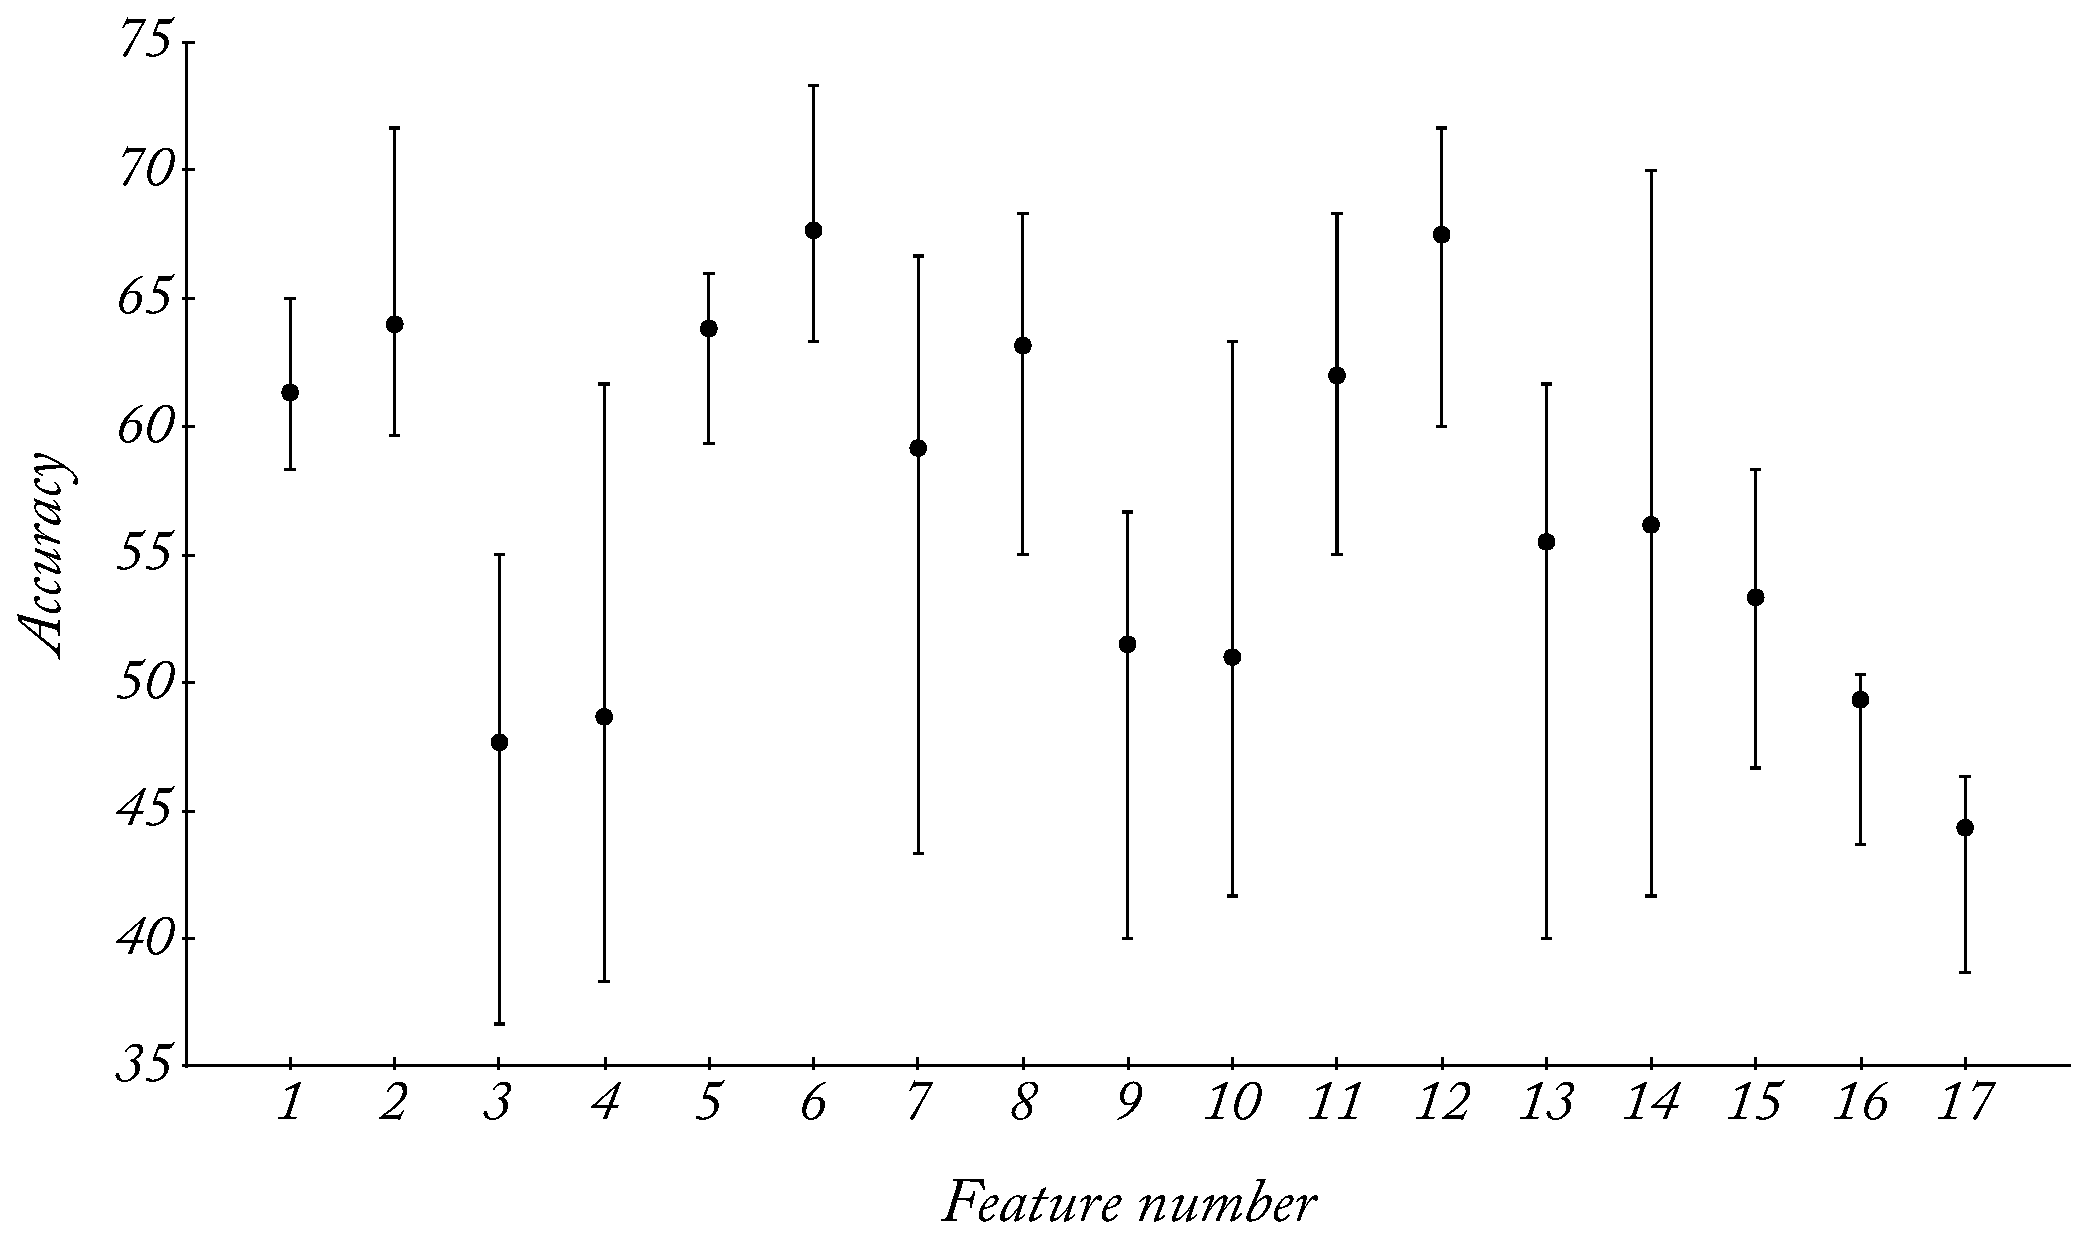
\includegraphics[width=1.0\textwidth]{graphs/polarity_a.pdf}
\end{figure}

\begin{figure}
	\caption{Individual figure accuracy}
	\label{fig:polarity_precision}
	\centering
		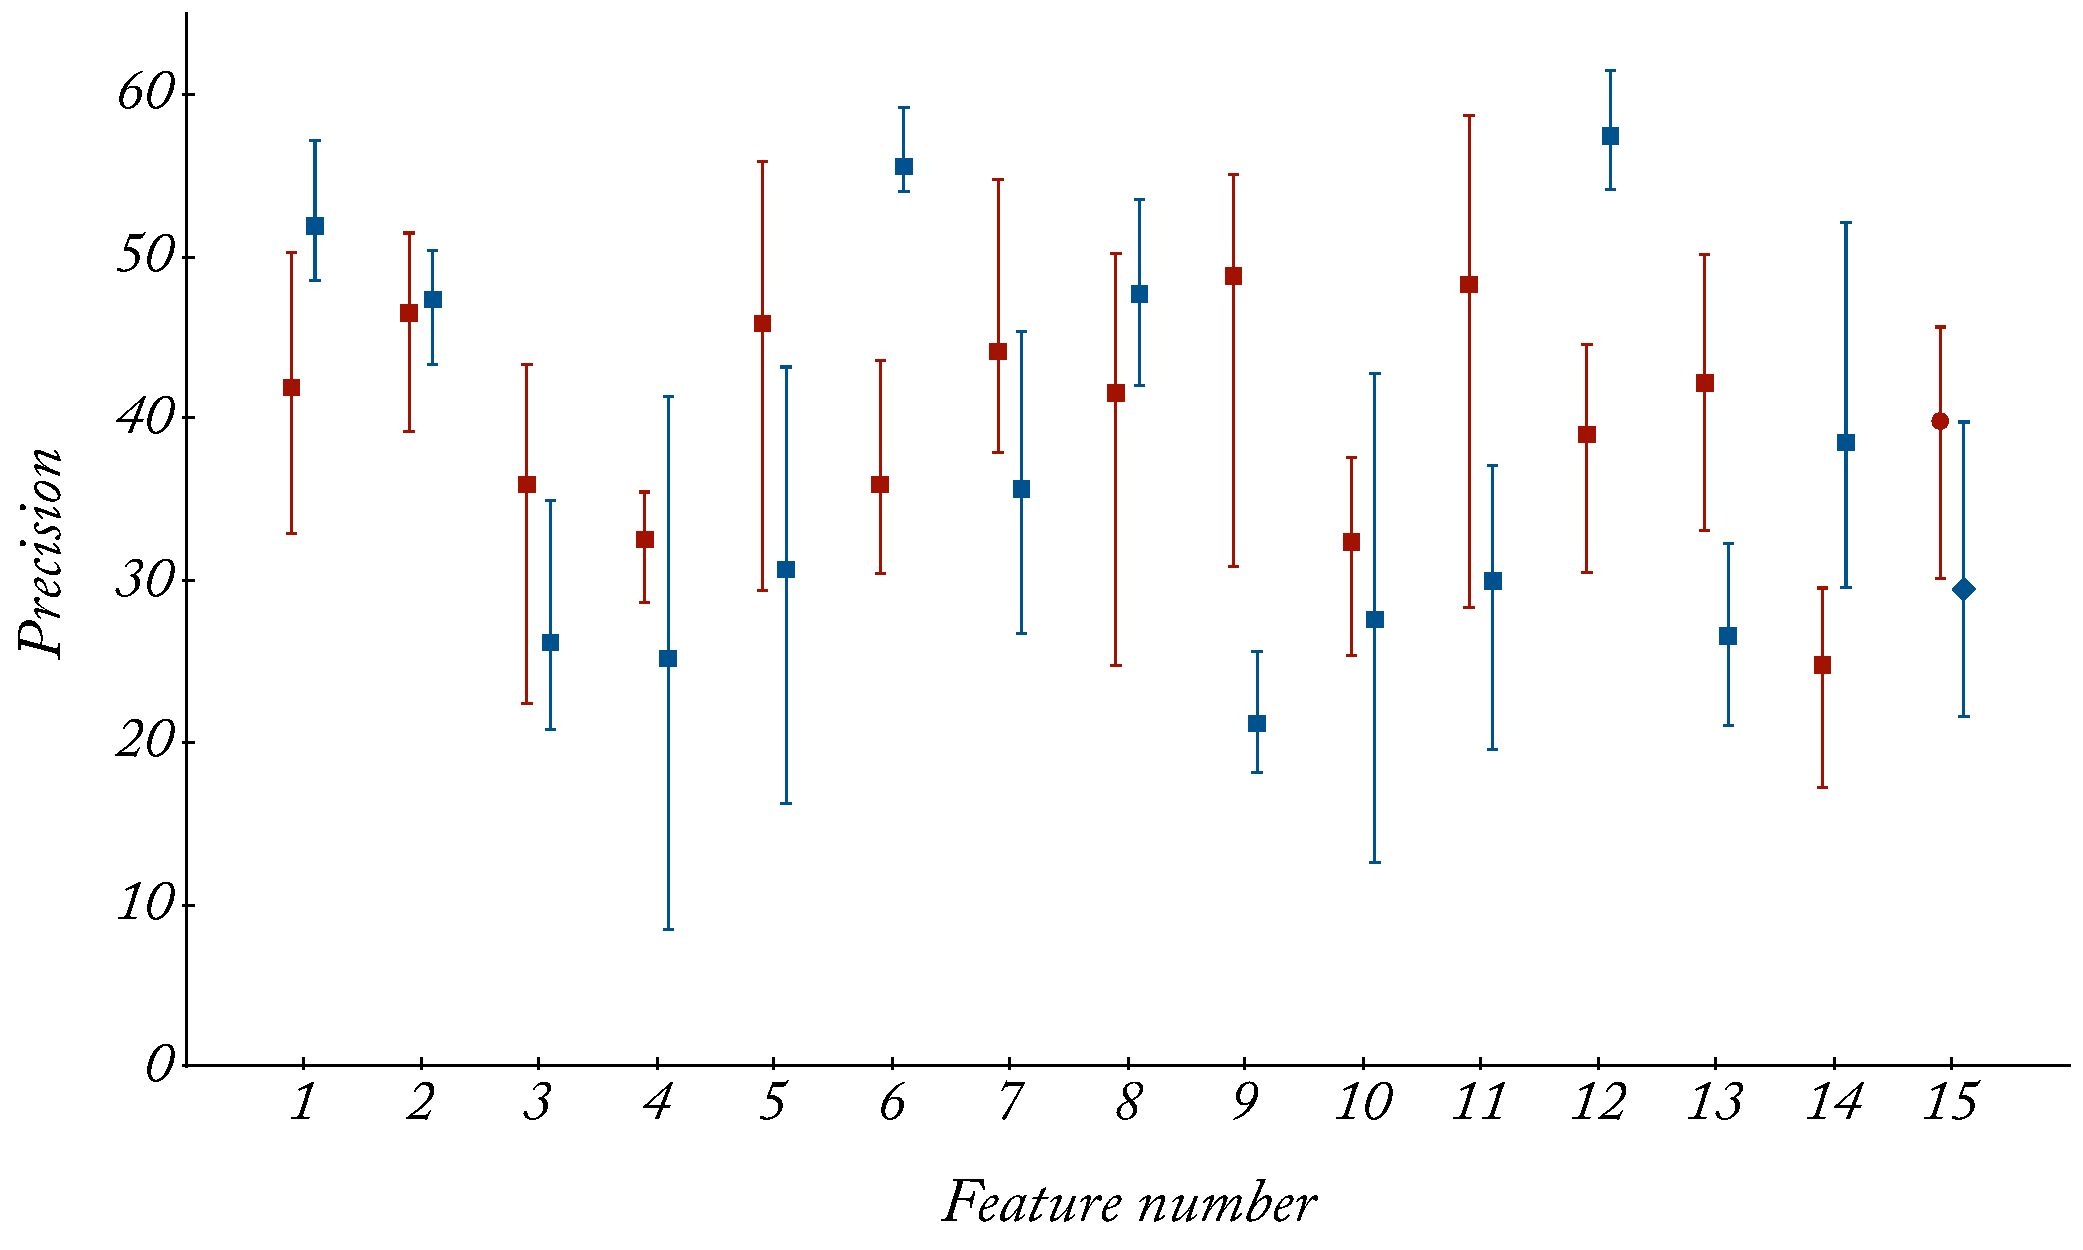
\includegraphics[width=1.0\textwidth]{graphs/polarity_p.pdf}
\end{figure}

\begin{figure}
	\caption{Individual figure accuracy}
	\label{fig:polarity_recall}
	\centering
		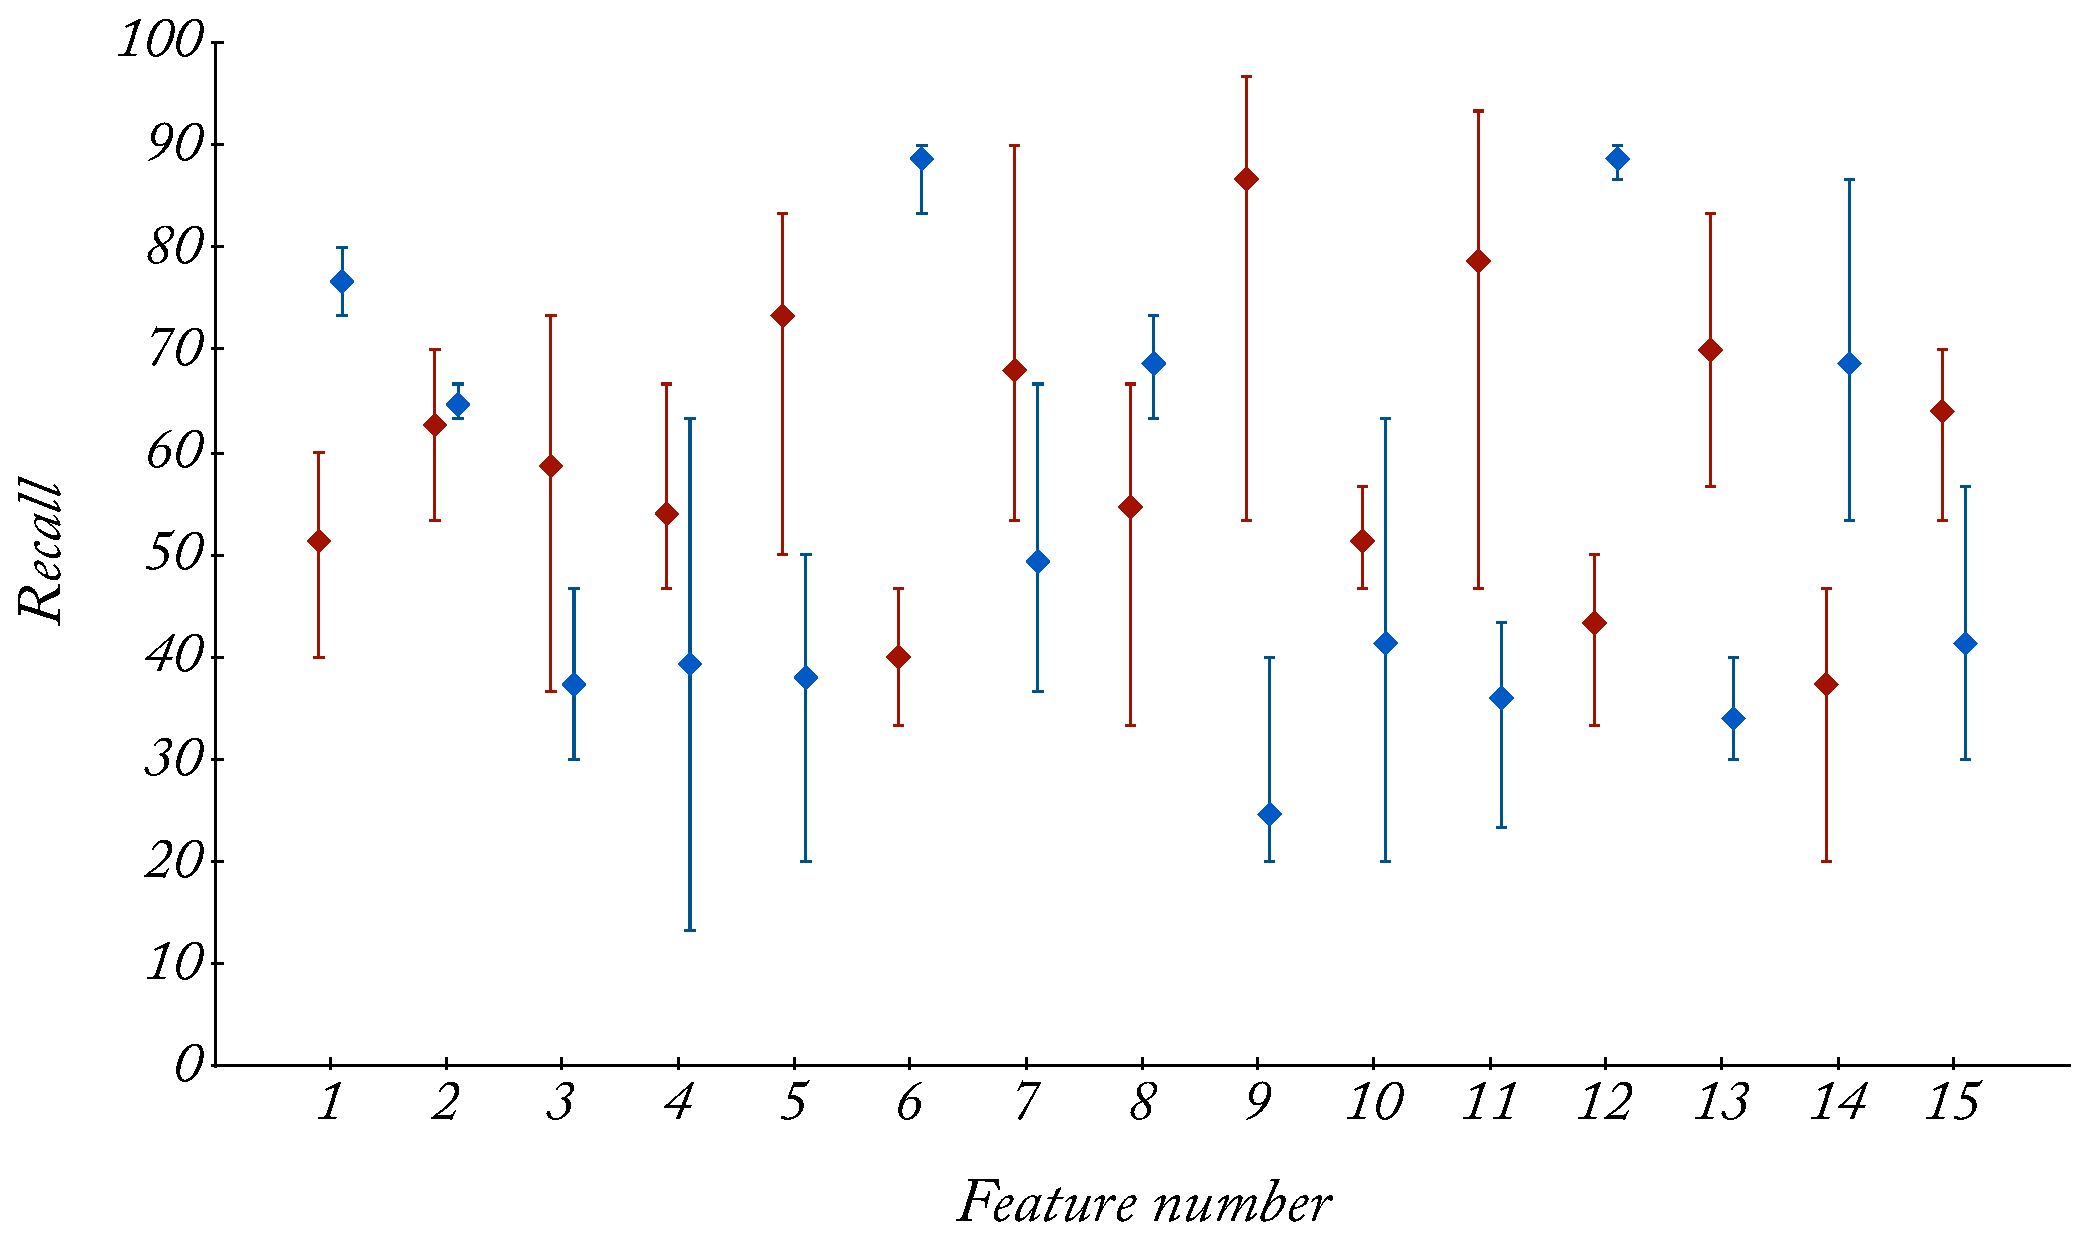
\includegraphics[width=1.0\textwidth]{graphs/polarity_r.pdf}
\end{figure}


\section{Evaluation}


